\documentclass[10pt]{beamer}

\usetheme[progressbar=frametitle]{metropolis}
\usepackage{appendixnumberbeamer}

\usepackage{booktabs}

%For linking email and website
\usepackage{hyperref}

%For enumeration as words
\usepackage{blindtext}
\usepackage{enumitem}

\usepackage{pgfplots}
\usepgfplotslibrary{dateplot}

\usepackage{xspace}
\newcommand{\themename}{\textbf{\textsc{metropolis}}\xspace}

\newcommand{\codeB}[1]{\texttt{#1}}

% Counter for the example and exercises
\newcounter{countexercise} % create a new counter
\newcounter{countexample}

\newcommand\showcountexercise{\stepcounter{countexercise}\thecountexercise}
\newcommand\showcounteample{\stepcounter{countexample}\thecountexample}


\title{Theory of Computation}
\subtitle{Tutorial 6 - Minimal DFAs}
\author{Cesare Spinoso-Di Piano}
\date{}

\begin{document}

\maketitle

\begin{frame}{Plan for today}
    \setbeamertemplate{section in toc}[sections numbered]
    \tableofcontents[hideallsubsections]
\end{frame}


\section{Minimal DFA}

\begin{frame}{Minimal DFA}
    Given a language $L$, there are several DFAs \textbf{M} that can accept it.\\ \bigskip
    \textbf{Theorem.} For every regular language $L$, there is a \textcolor{red}{unique} minimal DFA $\hat{M}$ that accepts it. $\hat{M}$ is minimal in the sense that no other DFA $M$ where $L(M) = L$ has a \underline{smaller} number of states.
\end{frame}

\begin{frame}[t]{State Reduction Algorithm}
    The following procedure takes as input any DFA $M = (Q, \Sigma, \delta, q_0, F)$ and outputs an equivalent minimal DFA $\hat{M} = (\hat{Q}, \Sigma, \hat{\delta}, \hat{q_0}, \hat{F})$ (i.e. $L(M) = L(\hat{M})$).
    \begin{itemize}
        \item Step 1. Remove all unreachable states from M.
        \item Step 2. Initialize two sets $S_1 \leftarrow Q - F$ and $S_2 \leftarrow F$.
        \item Step $j, (j > 2)$. For each pair $p, q \in S_i$
              \begin{itemize}
                  \item If $\delta(p, \sigma) \And \delta(q, \sigma)$ map to the same set $\forall \sigma \in \Sigma$, then $p,q$ are \underline{indistinguishable} and stay in the same set they were in Step $j-1$.
                  \item Otherwise, $p,q$ are \underline{distinguishable}, split the set from Step $j-1$ into two new sets one with $p$ and another with $q$. These sets may continue to grow.
                  \item If no new sets have been created from $j-1$ to $j$, end. Otherwise, continue.
              \end{itemize}
        \item $\hat{M}:$ Each set $S$ becomes a state in $\hat{Q}$. $\hat{q_0}$ is the set $S$ that contains $q_0$. $\hat{F}$ are the sets that contain at least one final state from $F$.
    \end{itemize}
\end{frame}

\begin{frame}[t]{Example}
    \textbf{Example \showcounteample{}.} Reduce the following $DFA$ \textbf{M}
    \begin{center}
        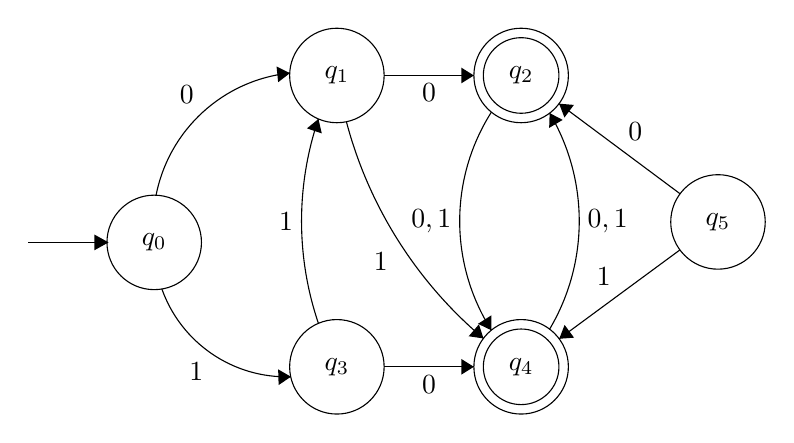
\begin{tikzpicture}[scale=0.2]
            \tikzstyle{every node}+=[inner sep=0pt]
            \draw [black] (11.8,-29.6) circle (3);
            \draw (11.8,-29.6) node {$q_0$};
            \draw [black] (23.4,-19) circle (3);
            \draw (23.4,-19) node {$q_1$};
            \draw [black] (35.1,-19) circle (3);
            \draw (35.1,-19) node {$q_2$};
            \draw [black] (35.1,-19) circle (2.4);
            \draw [black] (23.4,-37.5) circle (3);
            \draw (23.4,-37.5) node {$q_3$};
            \draw [black] (35.1,-37.5) circle (3);
            \draw (35.1,-37.5) node {$q_4$};
            \draw [black] (35.1,-37.5) circle (2.4);
            \draw [black] (47.6,-28.3) circle (3);
            \draw (47.6,-28.3) node {$q_5$};
            \draw [black] (45.19,-26.51) -- (37.51,-20.79);
            \fill [black] (37.51,-20.79) -- (37.85,-21.67) -- (38.45,-20.87);
            \draw (42.35,-23.15) node [above] {$0$};
            \draw [black] (45.18,-30.08) -- (37.52,-35.72);
            \fill [black] (37.52,-35.72) -- (38.46,-35.65) -- (37.86,-34.84);
            \draw (40.35,-32.4) node [above] {$1$};
            \draw [black] (33.213,-35.177) arc (-147.56206:-212.43794:12.914);
            \fill [black] (33.21,-35.18) -- (33.21,-34.23) -- (32.36,-34.77);
            \draw (30.7,-28.25) node [left] {$0,1$};
            \draw [black] (36.906,-21.388) arc (30.70302:-30.70302:13.44);
            \fill [black] (36.91,-21.39) -- (36.88,-22.33) -- (37.74,-21.82);
            \draw (39.29,-28.25) node [right] {$0,1$};
            \draw [black] (11.916,-26.614) arc (-191.09439:-264.0639:9.683);
            \fill [black] (20.42,-18.85) -- (19.57,-18.43) -- (19.67,-19.43);
            \draw (13.87,-20.84) node [above] {$0$};
            \draw [black] (20.483,-38.131) arc (-88.03497:-160.47745:8.397);
            \fill [black] (20.48,-38.13) -- (19.67,-37.66) -- (19.7,-38.66);
            \draw (14.47,-37.18) node [below] {$1$};
            \draw [black] (26.4,-37.5) -- (32.1,-37.5);
            \fill [black] (32.1,-37.5) -- (31.3,-37) -- (31.3,-38);
            \draw (29.25,-38) node [below] {$0$};
            \draw [black] (22.228,-34.742) arc (-161.23234:-198.76766:20.177);
            \fill [black] (22.23,-21.76) -- (21.5,-22.36) -- (22.44,-22.68);
            \draw (20.65,-28.25) node [left] {$1$};
            \draw [black] (26.4,-19) -- (32.1,-19);
            \fill [black] (32.1,-19) -- (31.3,-18.5) -- (31.3,-19.5);
            \draw (29.25,-19.5) node [below] {$0$};
            \draw [black] (32.705,-35.696) arc (-130.1762:-165.20263:27.048);
            \fill [black] (32.71,-35.7) -- (32.42,-34.8) -- (31.77,-35.56);
            \draw (26.67,-30.79) node [left] {$1$};
            \draw [black] (3.8,-29.6) -- (8.8,-29.6);
            \fill [black] (8.9, -29.6) -- (8.0, -30.1) -- (8.0, -29.1);

        \end{tikzpicture}
    \end{center}
\end{frame}

\begin{frame}[t]{Example}
    \textbf{Example 1.}
    \begin{itemize}
        \item Step 1: Remove all unreachable states from M.
        \item Step 2: Initialize two sets $S_1 \leftarrow \{q_0, q_1, q_3\}$, $S_2 \leftarrow \{q_2, q_4\}$
    \end{itemize}

    \begin{center}
        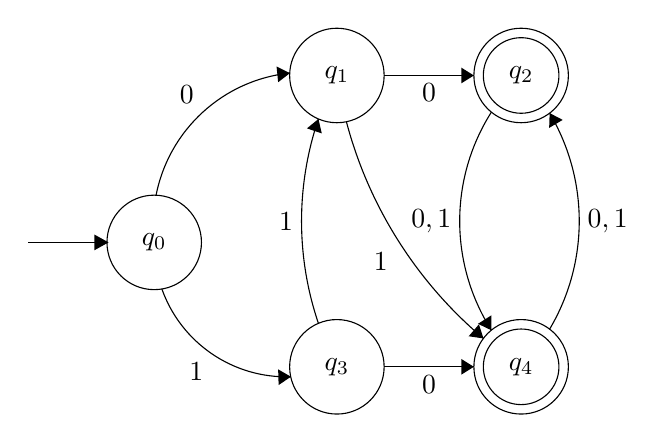
\begin{tikzpicture}[scale=0.2]
            \tikzstyle{every node}+=[inner sep=0pt]
            \draw [black] (11.8,-29.6) circle (3);
            \draw (11.8,-29.6) node {$q_0$};
            \draw [black] (23.4,-19) circle (3);
            \draw (23.4,-19) node {$q_1$};
            \draw [black] (35.1,-19) circle (3);
            \draw (35.1,-19) node {$q_2$};
            \draw [black] (35.1,-19) circle (2.4);
            \draw [black] (23.4,-37.5) circle (3);
            \draw (23.4,-37.5) node {$q_3$};
            \draw [black] (35.1,-37.5) circle (3);
            \draw (35.1,-37.5) node {$q_4$};
            \draw [black] (35.1,-37.5) circle (2.4);
            \draw [black] (33.213,-35.177) arc (-147.56206:-212.43794:12.914);
            \fill [black] (33.21,-35.18) -- (33.21,-34.23) -- (32.36,-34.77);
            \draw (30.7,-28.25) node [left] {$0,1$};
            \draw [black] (36.906,-21.388) arc (30.70302:-30.70302:13.44);
            \fill [black] (36.91,-21.39) -- (36.88,-22.33) -- (37.74,-21.82);
            \draw (39.29,-28.25) node [right] {$0,1$};
            \draw [black] (11.916,-26.614) arc (-191.09439:-264.0639:9.683);
            \fill [black] (20.42,-18.85) -- (19.57,-18.43) -- (19.67,-19.43);
            \draw (13.87,-20.84) node [above] {$0$};
            \draw [black] (20.483,-38.131) arc (-88.03497:-160.47745:8.397);
            \fill [black] (20.48,-38.13) -- (19.67,-37.66) -- (19.7,-38.66);
            \draw (14.47,-37.18) node [below] {$1$};
            \draw [black] (26.4,-37.5) -- (32.1,-37.5);
            \fill [black] (32.1,-37.5) -- (31.3,-37) -- (31.3,-38);
            \draw (29.25,-38) node [below] {$0$};
            \draw [black] (22.228,-34.742) arc (-161.23234:-198.76766:20.177);
            \fill [black] (22.23,-21.76) -- (21.5,-22.36) -- (22.44,-22.68);
            \draw (20.65,-28.25) node [left] {$1$};
            \draw [black] (26.4,-19) -- (32.1,-19);
            \fill [black] (32.1,-19) -- (31.3,-18.5) -- (31.3,-19.5);
            \draw (29.25,-19.5) node [below] {$0$};
            \draw [black] (32.705,-35.696) arc (-130.1762:-165.20263:27.048);
            \fill [black] (32.71,-35.7) -- (32.42,-34.8) -- (31.77,-35.56);
            \draw (26.67,-30.79) node [left] {$1$};
            \draw [black] (3.8,-29.6) -- (8.8,-29.6);
            \fill [black] (8.9, -29.6) -- (8.0, -30.1) -- (8.0, -29.1);
        \end{tikzpicture}
    \end{center}

\end{frame}

\begin{frame}[t]{Example}
    \textbf{Example 1.}
    \begin{itemize}
        \item Step j: Distinguishable and indistinguishable states
              \begin{itemize}
                  \item $\rightarrow \{q_0, q_1, q_3\}, \{q_2, q_4\}$
                  \item $\rightarrow \{q_0\} \{q_1\} \{q_3\} \{q_2, q_4\}$
                  \item $\rightarrow \{q_0\} \{q_1\} \{q_3\} \{q_2, q_4\}$\\
                        No change from previous step, states have been identified.
              \end{itemize}
    \end{itemize}

    \begin{center}
        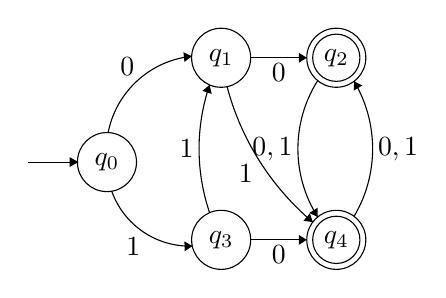
\begin{tikzpicture}[scale=0.125]
            \tikzstyle{every node}+=[inner sep=0pt]
            \draw [black] (11.8,-29.6) circle (3);
            \draw (11.8,-29.6) node {$q_0$};
            \draw [black] (23.4,-19) circle (3);
            \draw (23.4,-19) node {$q_1$};
            \draw [black] (35.1,-19) circle (3);
            \draw (35.1,-19) node {$q_2$};
            \draw [black] (35.1,-19) circle (2.4);
            \draw [black] (23.4,-37.5) circle (3);
            \draw (23.4,-37.5) node {$q_3$};
            \draw [black] (35.1,-37.5) circle (3);
            \draw (35.1,-37.5) node {$q_4$};
            \draw [black] (35.1,-37.5) circle (2.4);
            \draw [black] (33.213,-35.177) arc (-147.56206:-212.43794:12.914);
            \fill [black] (33.21,-35.18) -- (33.21,-34.23) -- (32.36,-34.77);
            \draw (30.7,-28.25) node [left] {$0,1$};
            \draw [black] (36.906,-21.388) arc (30.70302:-30.70302:13.44);
            \fill [black] (36.91,-21.39) -- (36.88,-22.33) -- (37.74,-21.82);
            \draw (39.29,-28.25) node [right] {$0,1$};
            \draw [black] (11.916,-26.614) arc (-191.09439:-264.0639:9.683);
            \fill [black] (20.42,-18.85) -- (19.57,-18.43) -- (19.67,-19.43);
            \draw (13.87,-20.84) node [above] {$0$};
            \draw [black] (20.483,-38.131) arc (-88.03497:-160.47745:8.397);
            \fill [black] (20.48,-38.13) -- (19.67,-37.66) -- (19.7,-38.66);
            \draw (14.47,-37.18) node [below] {$1$};
            \draw [black] (26.4,-37.5) -- (32.1,-37.5);
            \fill [black] (32.1,-37.5) -- (31.3,-37) -- (31.3,-38);
            \draw (29.25,-38) node [below] {$0$};
            \draw [black] (22.228,-34.742) arc (-161.23234:-198.76766:20.177);
            \fill [black] (22.23,-21.76) -- (21.5,-22.36) -- (22.44,-22.68);
            \draw (20.65,-28.25) node [left] {$1$};
            \draw [black] (26.4,-19) -- (32.1,-19);
            \fill [black] (32.1,-19) -- (31.3,-18.5) -- (31.3,-19.5);
            \draw (29.25,-19.5) node [below] {$0$};
            \draw [black] (32.705,-35.696) arc (-130.1762:-165.20263:27.048);
            \fill [black] (32.71,-35.7) -- (32.42,-34.8) -- (31.77,-35.56);
            \draw (26.67,-30.79) node [left] {$1$};
            \draw [black] (3.8,-29.6) -- (8.8,-29.6);
            \fill [black] (8.9, -29.6) -- (8.0, -30.1) -- (8.0, -29.1);
        \end{tikzpicture}
    \end{center}

\end{frame}


\begin{frame}[t]{Example}
    \textbf{Example 1.}
    \begin{itemize}
        \item Create $\hat{M}$: Each set $S$ becomes a state in $\hat{Q}$. $\hat{q_0}$ is the set $S$ that contains $q_0$. $\hat{F}$ are the sets that contain at least one final state from $F$.
    \end{itemize}
    \begin{center}
        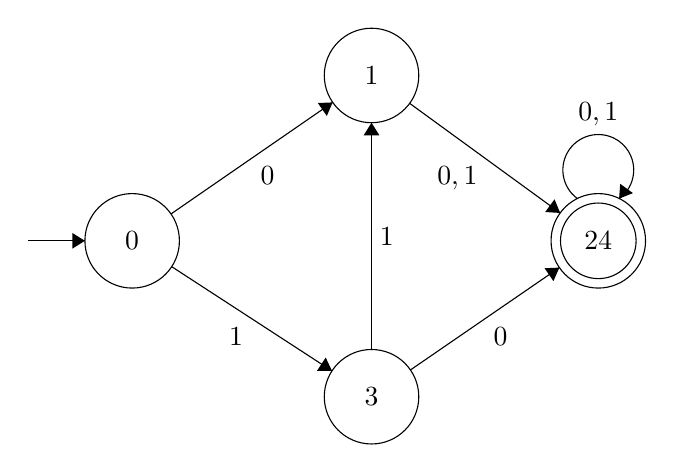
\begin{tikzpicture}[scale=0.2]
            \tikzstyle{every node}+=[inner sep=0pt]
            \draw [black] (11.8,-29.6) circle (3);
            \draw (11.8,-29.6) node {$0$};
            \draw [black] (27,-19.1) circle (3);
            \draw (27,-19.1) node {$1$};
            \draw [black] (27,-39.5) circle (3);
            \draw (27,-39.5) node {$3$};
            \draw [black] (41.4,-29.6) circle (3);
            \draw (41.4,-29.6) node {$24$};
            \draw [black] (41.4,-29.6) circle (2.4);
            \draw [black] (5.2,-29.6) -- (8.8,-29.6);
            \fill [black] (8.8,-29.6) -- (8,-29.1) -- (8,-30.1);
            \draw [black] (14.27,-27.89) -- (24.53,-20.81);
            \fill [black] (24.53,-20.81) -- (23.59,-20.85) -- (24.16,-21.67);
            \draw (20.4,-24.85) node [below] {$0$};
            \draw [black] (14.31,-31.24) -- (24.49,-37.86);
            \fill [black] (24.49,-37.86) -- (24.09,-37.01) -- (23.54,-37.85);
            \draw (18.4,-35.05) node [below] {$1$};
            \draw [black] (29.42,-20.87) -- (38.98,-27.83);
            \fill [black] (38.98,-27.83) -- (38.62,-26.96) -- (38.03,-27.77);
            \draw (32.45,-24.85) node [below] {$0,1$};
            \draw [black] (40.077,-26.92) arc (234:-54:2.25);
            \draw (41.4,-22.35) node [above] {$0,1$};
            \fill [black] (42.72,-26.92) -- (43.6,-26.57) -- (42.79,-25.98);
            \draw [black] (27,-36.5) -- (27,-22.1);
            \fill [black] (27,-22.1) -- (26.5,-22.9) -- (27.5,-22.9);
            \draw (27.5,-29.3) node [right] {$1$};
            \draw [black] (29.47,-37.8) -- (38.93,-31.3);
            \fill [black] (38.93,-31.3) -- (37.99,-31.34) -- (38.55,-32.16);
            \draw (35.2,-35.05) node [below] {$0$};
        \end{tikzpicture}
    \end{center}


\end{frame}

\begin{frame}[t]{Exercise}
    \textbf{Exercise \showcountexercise{}.} Minimize the DFA $M = (\{q_0,q_1,q_2,q_3,q_4,q_5\}, \{0,1\}, \delta, q_0, \{q_2,q_5\})$.  Where $\delta$ is given as:
    \begin{flushleft}
        \begin{tabular}{|c|c|c|}
            \hline
            $\delta$ & 0     & 1     \\ \hline
            $q_0$    & $q_1$ & $q_3$ \\ \hline
            $q_1$    & $q_1$ & $q_4$ \\ \hline
            $q_2$    & $q_0$ & $q_2$ \\ \hline
            $q_3$    & $q_3$ & $q_2$ \\ \hline
            $q_4$    & $q_4$ & $q_5$ \\ \hline
            $q_5$    & $q_0$ & $q_2$ \\ \hline
        \end{tabular}
    \end{flushleft}
\end{frame}

\end{document}

\begin{frame}[t]{Answer}
    \textbf{Exercise 1.} Minimize the DFA $M = (\{q_0,q_1,q_2,q_3,q_4,q_5\}, \{0,1\}, \delta, q_0, \{q_2,q_5\})$.\\\bigskip


    \begin{center}
        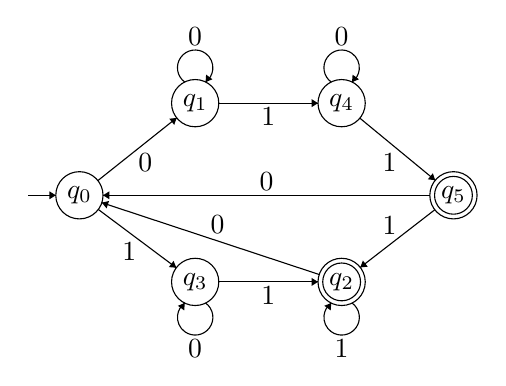
\begin{tikzpicture}[scale=0.1]
            \tikzstyle{every node}+=[inner sep=0pt]
            \draw [black] (12.9,-28.4) circle (3);
            \draw (12.9,-28.4) node {$q_0$};
            \draw [black] (27.6,-39.4) circle (3);
            \draw (27.6,-39.4) node {$q_3$};
            \draw [black] (27.6,-16.7) circle (3);
            \draw (27.6,-16.7) node {$q_1$};
            \draw [black] (46.2,-16.7) circle (3);
            \draw (46.2,-16.7) node {$q_4$};
            \draw [black] (46.2,-39.4) circle (3);
            \draw (46.2,-39.4) node {$q_2$};
            \draw [black] (46.2,-39.4) circle (2.4);
            \draw [black] (60.4,-28.4) circle (3);
            \draw (60.4,-28.4) node {$q_5$};
            \draw [black] (60.4,-28.4) circle (2.4);
            \draw [black] (6.4,-28.4) -- (9.9,-28.4);
            \fill [black] (9.9,-28.4) -- (9.1,-27.9) -- (9.1,-28.9);
            \draw [black] (15.3,-30.2) -- (25.2,-37.6);
            \fill [black] (25.2,-37.6) -- (24.86,-36.72) -- (24.26,-37.52);
            \draw (19.25,-34.4) node [below] {$1$};
            \draw [black] (15.25,-26.53) -- (25.25,-18.57);
            \fill [black] (25.25,-18.57) -- (24.32,-18.68) -- (24.94,-19.46);
            \draw (21.26,-23.04) node [below] {$0$};
            \draw [black] (26.277,-14.02) arc (234:-54:2.25);
            \draw (27.6,-9.45) node [above] {$0$};
            \fill [black] (28.92,-14.02) -- (29.8,-13.67) -- (28.99,-13.08);
            \draw [black] (28.923,-42.08) arc (54:-234:2.25);
            \draw (27.6,-46.65) node [below] {$0$};
            \fill [black] (26.28,-42.08) -- (25.4,-42.43) -- (26.21,-43.02);
            \draw [black] (30.6,-39.4) -- (43.2,-39.4);
            \fill [black] (43.2,-39.4) -- (42.4,-38.9) -- (42.4,-39.9);
            \draw (36.9,-39.9) node [below] {$1$};
            \draw [black] (47.523,-42.08) arc (54:-234:2.25);
            \draw (46.2,-46.65) node [below] {$1$};
            \fill [black] (44.88,-42.08) -- (44,-42.43) -- (44.81,-43.02);
            \draw [black] (58.03,-30.24) -- (48.57,-37.56);
            \fill [black] (48.57,-37.56) -- (49.51,-37.47) -- (48.9,-36.68);
            \draw (52.29,-33.4) node [above] {$1$};
            \draw [black] (48.52,-18.61) -- (58.08,-26.49);
            \fill [black] (58.08,-26.49) -- (57.79,-25.6) -- (57.15,-26.37);
            \draw (52.29,-23.04) node [below] {$1$};
            \draw [black] (44.877,-14.02) arc (234:-54:2.25);
            \draw (46.2,-9.45) node [above] {$0$};
            \fill [black] (47.52,-14.02) -- (48.4,-13.67) -- (47.59,-13.08);
            \draw [black] (30.6,-16.7) -- (43.2,-16.7);
            \fill [black] (43.2,-16.7) -- (42.4,-16.2) -- (42.4,-17.2);
            \draw (36.9,-17.2) node [below] {$1$};
            \draw [black] (57.4,-28.4) -- (15.9,-28.4);
            \fill [black] (15.9,-28.4) -- (16.7,-28.9) -- (16.7,-27.9);
            \draw (36.65,-27.9) node [above] {$0$};
            \draw [black] (43.35,-38.46) -- (15.75,-29.34);
            \fill [black] (15.75,-29.34) -- (16.35,-30.07) -- (16.67,-29.12);
            \draw (30.44,-33.36) node [above] {$0$};
        \end{tikzpicture}
    \end{center}
    \begin{itemize}
        \item Step 1. \textcolor{red}{There are no unreachable states. Nothing to do in this step.}
        \item Step 2. \textcolor{red}{$S_1 \leftarrow \{q_0,q_1,q_3,q_4\}, S_2 \leftarrow \{q_2, q_5\}$}
    \end{itemize}




\end{frame}

\begin{frame}[t]{Answer (Continued)}
    \textbf{Exercise 1.} Minimize the DFA $M = (\{q_0,q_1,q_2,q_3,q_4,q_5\}, \{0,1\}, \delta, q_0, \{q_2,q_5\})$.\\\bigskip

    \begin{itemize}
        \item Step j.
              \begin{itemize}
                  \item 1. \textcolor{red}{$\{q_0,q_1,q_3,q_4\}, \{q_2, q_5\}$}
                  \item 2. \textcolor{red}{$\{q_0,q_1\}, \{q_3,q_4\}, \{q_2, q_5\}$}
                  \item 3. \textcolor{red}{$\{q_0,q_1\}, \{q_3,q_4\}, \{q_2, q_5\}$. No change, states have been identified.}
              \end{itemize}
        \item Build minimal DFA
    \end{itemize}
    \begin{center}

        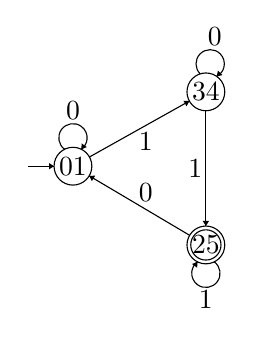
\begin{tikzpicture}[scale=0.08]
            \tikzstyle{every node}+=[inner sep=0pt]
            \draw [black] (13.3,-27.6) circle (3);
            \draw (13.3,-27.6) node {$01$};
            \draw [black] (34.4,-15.8) circle (3);
            \draw (34.4,-15.8) node {$34$};
            \draw [black] (34.4,-40.1) circle (3);
            \draw (34.4,-40.1) node {$25$};
            \draw [black] (34.4,-40.1) circle (2.4);
            \draw [black] (6.2,-27.6) -- (10.3,-27.6);
            \fill [black] (10.3,-27.6) -- (9.5,-27.1) -- (9.5,-28.1);
            \draw [black] (11.977,-24.92) arc (234:-54:2.25);
            \draw (13.3,-20.35) node [above] {$0$};
            \fill [black] (14.62,-24.92) -- (15.5,-24.57) -- (14.69,-23.98);
            \draw [black] (15.92,-26.14) -- (31.78,-17.26);
            \fill [black] (31.78,-17.26) -- (30.84,-17.22) -- (31.33,-18.09);
            \draw (24.85,-22.2) node [below] {$1$};
            \draw [black] (33.5,-12.951) arc (225.26887:-62.73113:2.25);
            \draw (35.81,-8.53) node [above] {$0$};
            \fill [black] (36.11,-13.35) -- (37.03,-13.14) -- (36.32,-12.43);
            \draw [black] (34.4,-18.8) -- (34.4,-37.1);
            \fill [black] (34.4,-37.1) -- (34.9,-36.3) -- (33.9,-36.3);
            \draw (33.9,-27.95) node [left] {$1$};
            \draw [black] (31.82,-38.57) -- (15.88,-29.13);
            \fill [black] (15.88,-29.13) -- (16.31,-29.97) -- (16.82,-29.11);
            \draw (24.85,-33.35) node [above] {$0$};
            \draw [black] (35.723,-42.78) arc (54:-234:2.25);
            \draw (34.4,-47.35) node [below] {$1$};
            \fill [black] (33.08,-42.78) -- (32.2,-43.13) -- (33.01,-43.72);
        \end{tikzpicture}

    \end{center}




\end{frame}

\begin{frame}[t]{Exercise}
    \textbf{Exercise \showcountexercise{}.} Find a minimal DFA $M$ for the language $L = \{b,ba\} \cup \{a^nb: n > 0\}$.
\end{frame}

\begin{frame}[t]{Answer}
    \textbf{Exercise 2.} Find a minimal DFA $M$ for the language $L = \{b,ba\} \cup \{a^nb: n > 0\}$. \textcolor{red}{Build a DFA for this language and then apply the minimization algorithm. Only the final minimal DFA is given here.}
    \begin{center}
        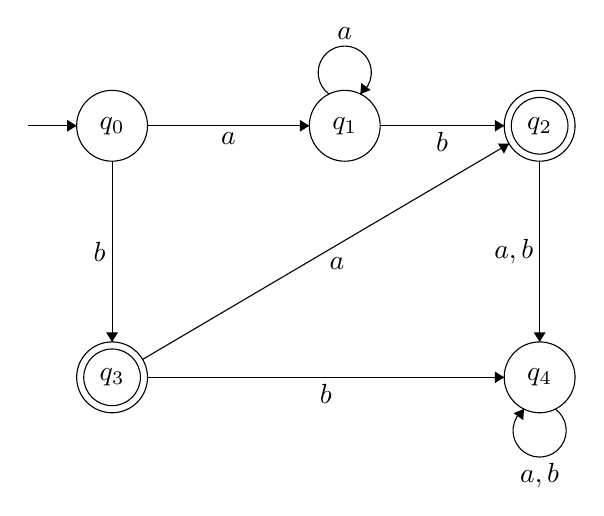
\begin{tikzpicture}[scale=0.15]
            \tikzstyle{every node}+=[inner sep=0pt]
            \draw [black] (14.8,-26.4) circle (3);
            \draw (14.8,-26.4) node {$q_0$};
            \draw [black] (34.5,-26.4) circle (3);
            \draw (34.5,-26.4) node {$q_1$};
            \draw [black] (51,-26.4) circle (3);
            \draw (51,-26.4) node {$q_2$};
            \draw [black] (51,-26.4) circle (2.4);
            \draw [black] (14.8,-47.7) circle (3);
            \draw (14.8,-47.7) node {$q_3$};
            \draw [black] (14.8,-47.7) circle (2.4);
            \draw [black] (51,-47.7) circle (3);
            \draw (51,-47.7) node {$q_4$};
            \draw [black] (7.7,-26.4) -- (11.8,-26.4);
            \fill [black] (11.8,-26.4) -- (11,-25.9) -- (11,-26.9);
            \draw [black] (17.8,-26.4) -- (31.5,-26.4);
            \fill [black] (31.5,-26.4) -- (30.7,-25.9) -- (30.7,-26.9);
            \draw (24.65,-26.9) node [below] {$a$};
            \draw [black] (14.8,-29.4) -- (14.8,-44.7);
            \fill [black] (14.8,-44.7) -- (15.3,-43.9) -- (14.3,-43.9);
            \draw (14.3,-37.05) node [left] {$b$};
            \draw [black] (33.177,-23.72) arc (234:-54:2.25);
            \draw (34.5,-19.15) node [above] {$a$};
            \fill [black] (35.82,-23.72) -- (36.7,-23.37) -- (35.89,-22.78);
            \draw [black] (37.5,-26.4) -- (48,-26.4);
            \fill [black] (48,-26.4) -- (47.2,-25.9) -- (47.2,-26.9);
            \draw (42.75,-26.9) node [below] {$b$};
            \draw [black] (17.39,-46.18) -- (48.41,-27.92);
            \fill [black] (48.41,-27.92) -- (47.47,-27.9) -- (47.98,-28.76);
            \draw (33.84,-37.55) node [below] {$a$};
            \draw [black] (51,-29.4) -- (51,-44.7);
            \fill [black] (51,-44.7) -- (51.5,-43.9) -- (50.5,-43.9);
            \draw (50.5,-37.05) node [left] {$a,b$};
            \draw [black] (52.323,-50.38) arc (54:-234:2.25);
            \draw (51,-54.95) node [below] {$a,b$};
            \fill [black] (49.68,-50.38) -- (48.8,-50.73) -- (49.61,-51.32);
            \draw [black] (17.8,-47.7) -- (48,-47.7);
            \fill [black] (48,-47.7) -- (47.2,-47.2) -- (47.2,-48.2);
            \draw (32.9,-48.2) node [below] {$b$};
        \end{tikzpicture}
    \end{center}
\end{frame}



